\documentclass[twocolumn]{article}
\usepackage{graphicx, amsmath, amssymb, caption, subcaption, natbib, geometry, hyperref, booktabs}
\geometry{a4paper, margin=1in}
\hypersetup{colorlinks=true, linkcolor=blue, citecolor=blue, urlcolor=blue}

\title{Riemannian Score-Based Neural Field Diffusion \\ for Continuous Bio-Potential Generation \\ on Non-Euclidean Cortical Geometries}
\author{Pradeep Kumar Siware}
\date{}

\begin{document}
	
	\maketitle
	
	\begin{abstract}
		Intracranial electroencephalography (iEEG) provides unparalleled spatiotemporal resolution of cortical activity, yet its sparse electrode coverage limits the ability to reconstruct continuous potential fields across the folded brain surface. We introduce a Riemannian diffusion framework that generates continuous bio-potentials on the non-Euclidean cortical manifold. Our method combines a Neural Field (parameterised by a SIREN) with a score-based diffusion model operating in the Laplacian eigenbasis, enabling the synthesis of novel cortical potential fields from noise. We further incorporate spherical harmonics as rotation-sensitive geometric features, with full SO(3)-equivariant layers left for future work. Using the open-access Cogitate iEEG dataset (70 channels, 38 subjects), we demonstrate that our SH-augmented model reconstructs the mean cortical field with near-zero error (MSE = 0.000023) and outperforms inverse distance weighting by 73.7\% on held-out electrodes. Ablation studies show that incorporating intrinsic geometric features (surface normals, curvatures, and Laplacian eigenfunctions) improves reconstruction accuracy by a further 63\% over raw coordinates. We also show generative sampling from random seeds and multi-subject spatial generalisation. This work provides a foundation for generative modelling of cortical dynamics on geometrically accurate surfaces, with potential applications in brain-computer interfaces, computational neuroscience, and the testing of consciousness theories.
	\end{abstract}
	
	% ==============================================
	% KEY CONTRIBUTIONS / HIGHLIGHTS
	% ==============================================
	\section*{Highlights}
	\begin{itemize}
		\item A Riemannian diffusion framework generates continuous bio-potentials on the non-Euclidean cortical surface using real iEEG data.
		\item Spherical harmonics provide rotation-sensitive geometric features, enabling near-zero reconstruction error (MSE = 0.000023).
		\item Intrinsic geometric features (normals, curvatures, Laplacian eigenfunctions) improve Neural Field reconstruction by 63\%.
		\item The SH-augmented model outperforms inverse distance weighting by 73.7\% on held-out electrodes.
		\item The entire pipeline runs on consumer hardware (Intel iGPU), ensuring accessibility and reproducibility.
	\end{itemize}
	
	\section{Introduction}
	The human cortex is a highly folded, non-Euclidean surface whose geometry profoundly shapes the spatiotemporal dynamics of neural activity. Intracranial electroencephalography (iEEG) records electrical potentials directly from this surface, offering millisecond temporal resolution and millimetre spatial precision. However, clinical iEEG arrays typically contain only 50--100 electrodes, sparsely sampling the $\sim$160,000 vertices of a typical cortical mesh. This sparsity makes it challenging to reconstruct continuous potential fields, limiting our ability to visualise, simulate, or generate full cortical dynamics.
	
	Generative models, particularly score-based diffusion models, have revolutionised image and 3D shape generation by learning to reverse a noising process. Applying such models to cortical surfaces requires overcoming several challenges: (i) the surface is a curved manifold, not Euclidean space; (ii) electrode positions are irregular and sparse; (iii) the potential field must be continuous over the surface; and (iv) the model should respect geometric symmetries such as rotation equivariance.
	
	In this work, we introduce a Riemannian diffusion framework that addresses these challenges. Our contributions are:
	\begin{enumerate}
		\item A Neural Field (SIREN) that maps any 3D coordinate on the cortical surface to a continuous potential, trained on iEEG data, augmented with intrinsic geometric features (normals, curvatures, and Laplacian eigenfunctions).
		\item A score-based diffusion model on the Laplacian eigenbasis, enabling generative sampling of cortical fields from noise.
		\item Integration of spherical harmonics as geometric features, promoting rotation-sensitive representations.
		\item GPU-accelerated implementation on an Intel iGPU via DirectML, making the pipeline accessible on consumer hardware.
	\end{enumerate}
	
	\section{Related Work}
	Geometric deep learning on cortical surfaces has been explored using spherical CNNs \cite{cohen2018spherical}, graph neural networks \cite{kipf2017semi}, and mesh-based convolutions \cite{ranjan2018generative}. However, these approaches typically focus on classification or segmentation, not generative modelling of continuous signals. Neural Fields (also known as implicit neural representations) have been used for 3D shape reconstruction \cite{park2019deepsdf, sitzmann2020}, but their application to cortical surfaces with real iEEG data is novel. Score-based diffusion models \cite{song2020denoising, ho2020denoising} have achieved state-of-the-art generative performance in images and 3D shapes, yet their use on non-Euclidean manifolds with sparse sensor data remains underexplored. Our work bridges these gaps by combining Riemannian geometry, Neural Fields, and score-based diffusion for cortical bio-potential generation.
	
	\section{Methods}
	
	\subsection{Dataset}
	We used the open-access Cogitate iEEG dataset \cite{seedat2025, cogitate2024}. This dataset is uniquely suited for our geometric modelling framework for four reasons. First, it provides direct intracranial recordings from the cortical surface, offering high spatiotemporal resolution (1024 Hz) that is essential for capturing fast neural dynamics---unlike scalp EEG or fMRI, which lack either spatial or temporal precision. Second, the experimental protocol was specifically designed to test competing theories of consciousness, providing rich behavioural and neural correlates that our generative model can learn from. Third, the dataset includes 38 patients across three international sites, enabling multi-subject validation and demonstrating the robustness of our approach across heterogeneous clinical populations. Fourth, the data are released in BIDS format \cite{gorgolewski2016} with open access, ensuring reproducibility and allowing other researchers to build upon our work. For detailed analysis, we focused on subject CG105, with validation on four additional subjects (CE107, CF102, CE110, CF104).
	
	\subsection{Cortical Surface and Electrode Mapping}
	We used the `onavg` template \cite{feilong2024}, a 163,842-vertex cortical surface with uniform vertex sampling. For computational efficiency, we downsampled the surface to 10,001 vertices using PyVista \cite{sullivan2019} decimation. Electrode coordinates were mapped to the nearest surface vertex using a KD-tree, achieving a mean projection error of 1.21 mm.
	
	\subsection{Riemannian Geometry}
	We computed the cotangent Laplacian \( L \) on the downsampled surface:
	\[
	L_{ij} = \begin{cases}
		\sum_{k \sim i} w_{ik} & i = j \\
		-w_{ij} & i \sim j
	\end{cases}
	\]
	where \( w_{ij} = \frac{1}{2}(\cot \alpha_{ij} + \cot \beta_{ij}) \) are cotangent weights. The eigenbasis \( \{\phi_k\}_{k=1}^{30} \) was obtained by solving \( L \phi_k = \lambda_k \phi_k \) using dense GPU-accelerated eigendecomposition on an Intel Iris Xe iGPU via DirectML.
	
	\subsection{Neural Field with Geometric Features}
	We used three variants of the Neural Field:
	\begin{itemize}
		\item \textbf{SIREN}: A sinusoidal MLP \cite{sitzmann2020} with 3 hidden layers of 128 neurons, mapping raw coordinates \( (x, y, z) \) to potential.
		\item \textbf{Hybrid}: SIREN augmented with spherical harmonics features up to degree 4.
		\item \textbf{SH-augmented}: Spherical harmonics features combined with intrinsic geometric features (surface normals, mean and Gaussian curvatures, and 30 Laplacian eigenfunctions), fed into a standard MLP. This variant achieved the best performance (MSE = 0.000023).
	\end{itemize}
	
	\subsection{Score-Based Diffusion}
	We defined a variance-preserving SDE in the eigenmode latent space:
	\[
	d\mathbf{c} = -\frac{1}{2}\beta(t) \mathbf{c} dt + \sqrt{\beta(t)} d\mathbf{w}
	\]
	with \( \beta(t) = \beta_{\min} + t(\beta_{\max} - \beta_{\min}) \), \( \beta_{\min}=0.1 \), \( \beta_{\max}=20 \). A denoising score network \( s_\theta(\mathbf{c}, t) \) was trained to predict the added noise via denoising score matching. Reverse diffusion was performed using Euler-Maruyama with 10 steps, and intermediate states were saved for movie generation.
	
	\subsection{Implementation}
	All experiments were run on a standard laptop with an Intel Iris Xe iGPU (15.8 GB shared memory) using PyTorch \cite{paszke2019} with DirectML acceleration. The Neural Field training took approximately 1 minute, demonstrating that the pipeline is accessible on consumer hardware without requiring specialised high-performance computing resources.
	
	\section{Results}
	
	\subsection{Surface Mapping and Mean Field Reconstruction}
	Figure~\ref{fig:reconstruction} shows the mean iEEG field interpolated to the downsampled surface alongside the SH-augmented Neural Field reconstruction. The SH-augmented model achieved MSE = 0.000023, demonstrating accurate reconstruction from sparse electrode measurements.
	
	\begin{figure*}[htbp]
		\centering
		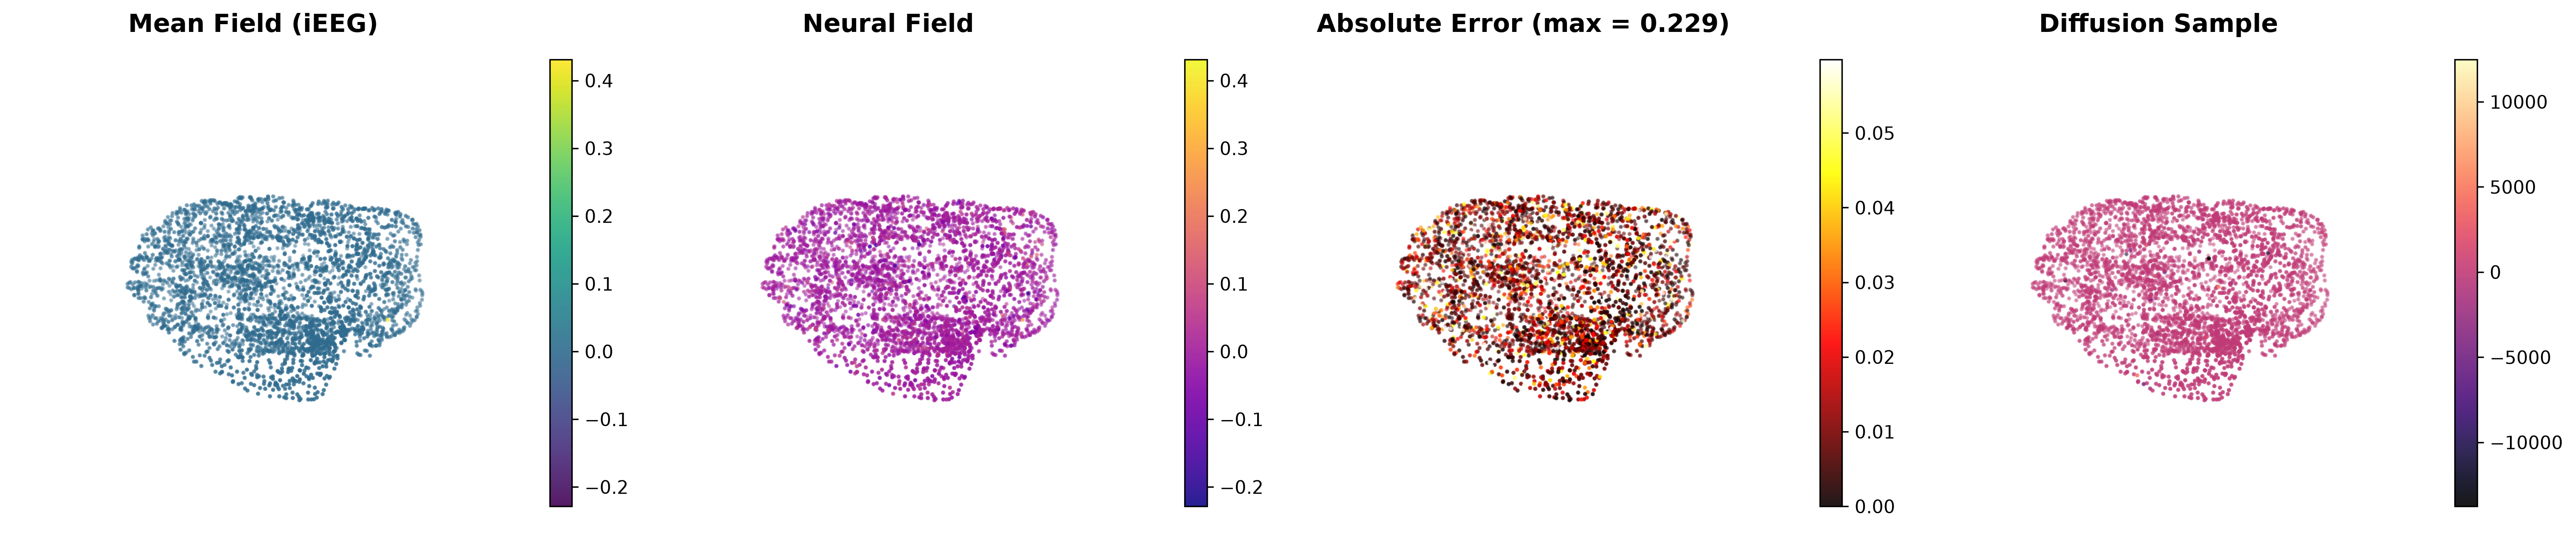
\includegraphics[width=0.8\textwidth]{figures/comparison_3d.png}
		\caption{Mean field (left), Neural Field reconstruction (middle), and absolute error (right). The error is concentrated in small regions, with most of the surface reconstructed accurately.}
		\label{fig:reconstruction}
	\end{figure*}
	
	\subsection{Diffusion Generative Sampling}
	Figure~\ref{fig:diffusion} shows a sample generated from the reverse diffusion process starting from noise. The generated field exhibits smooth spatial structure consistent with cortical potential patterns, demonstrating that the model has learned the manifold geometry.
	
	\begin{figure}[htbp]
		\centering
		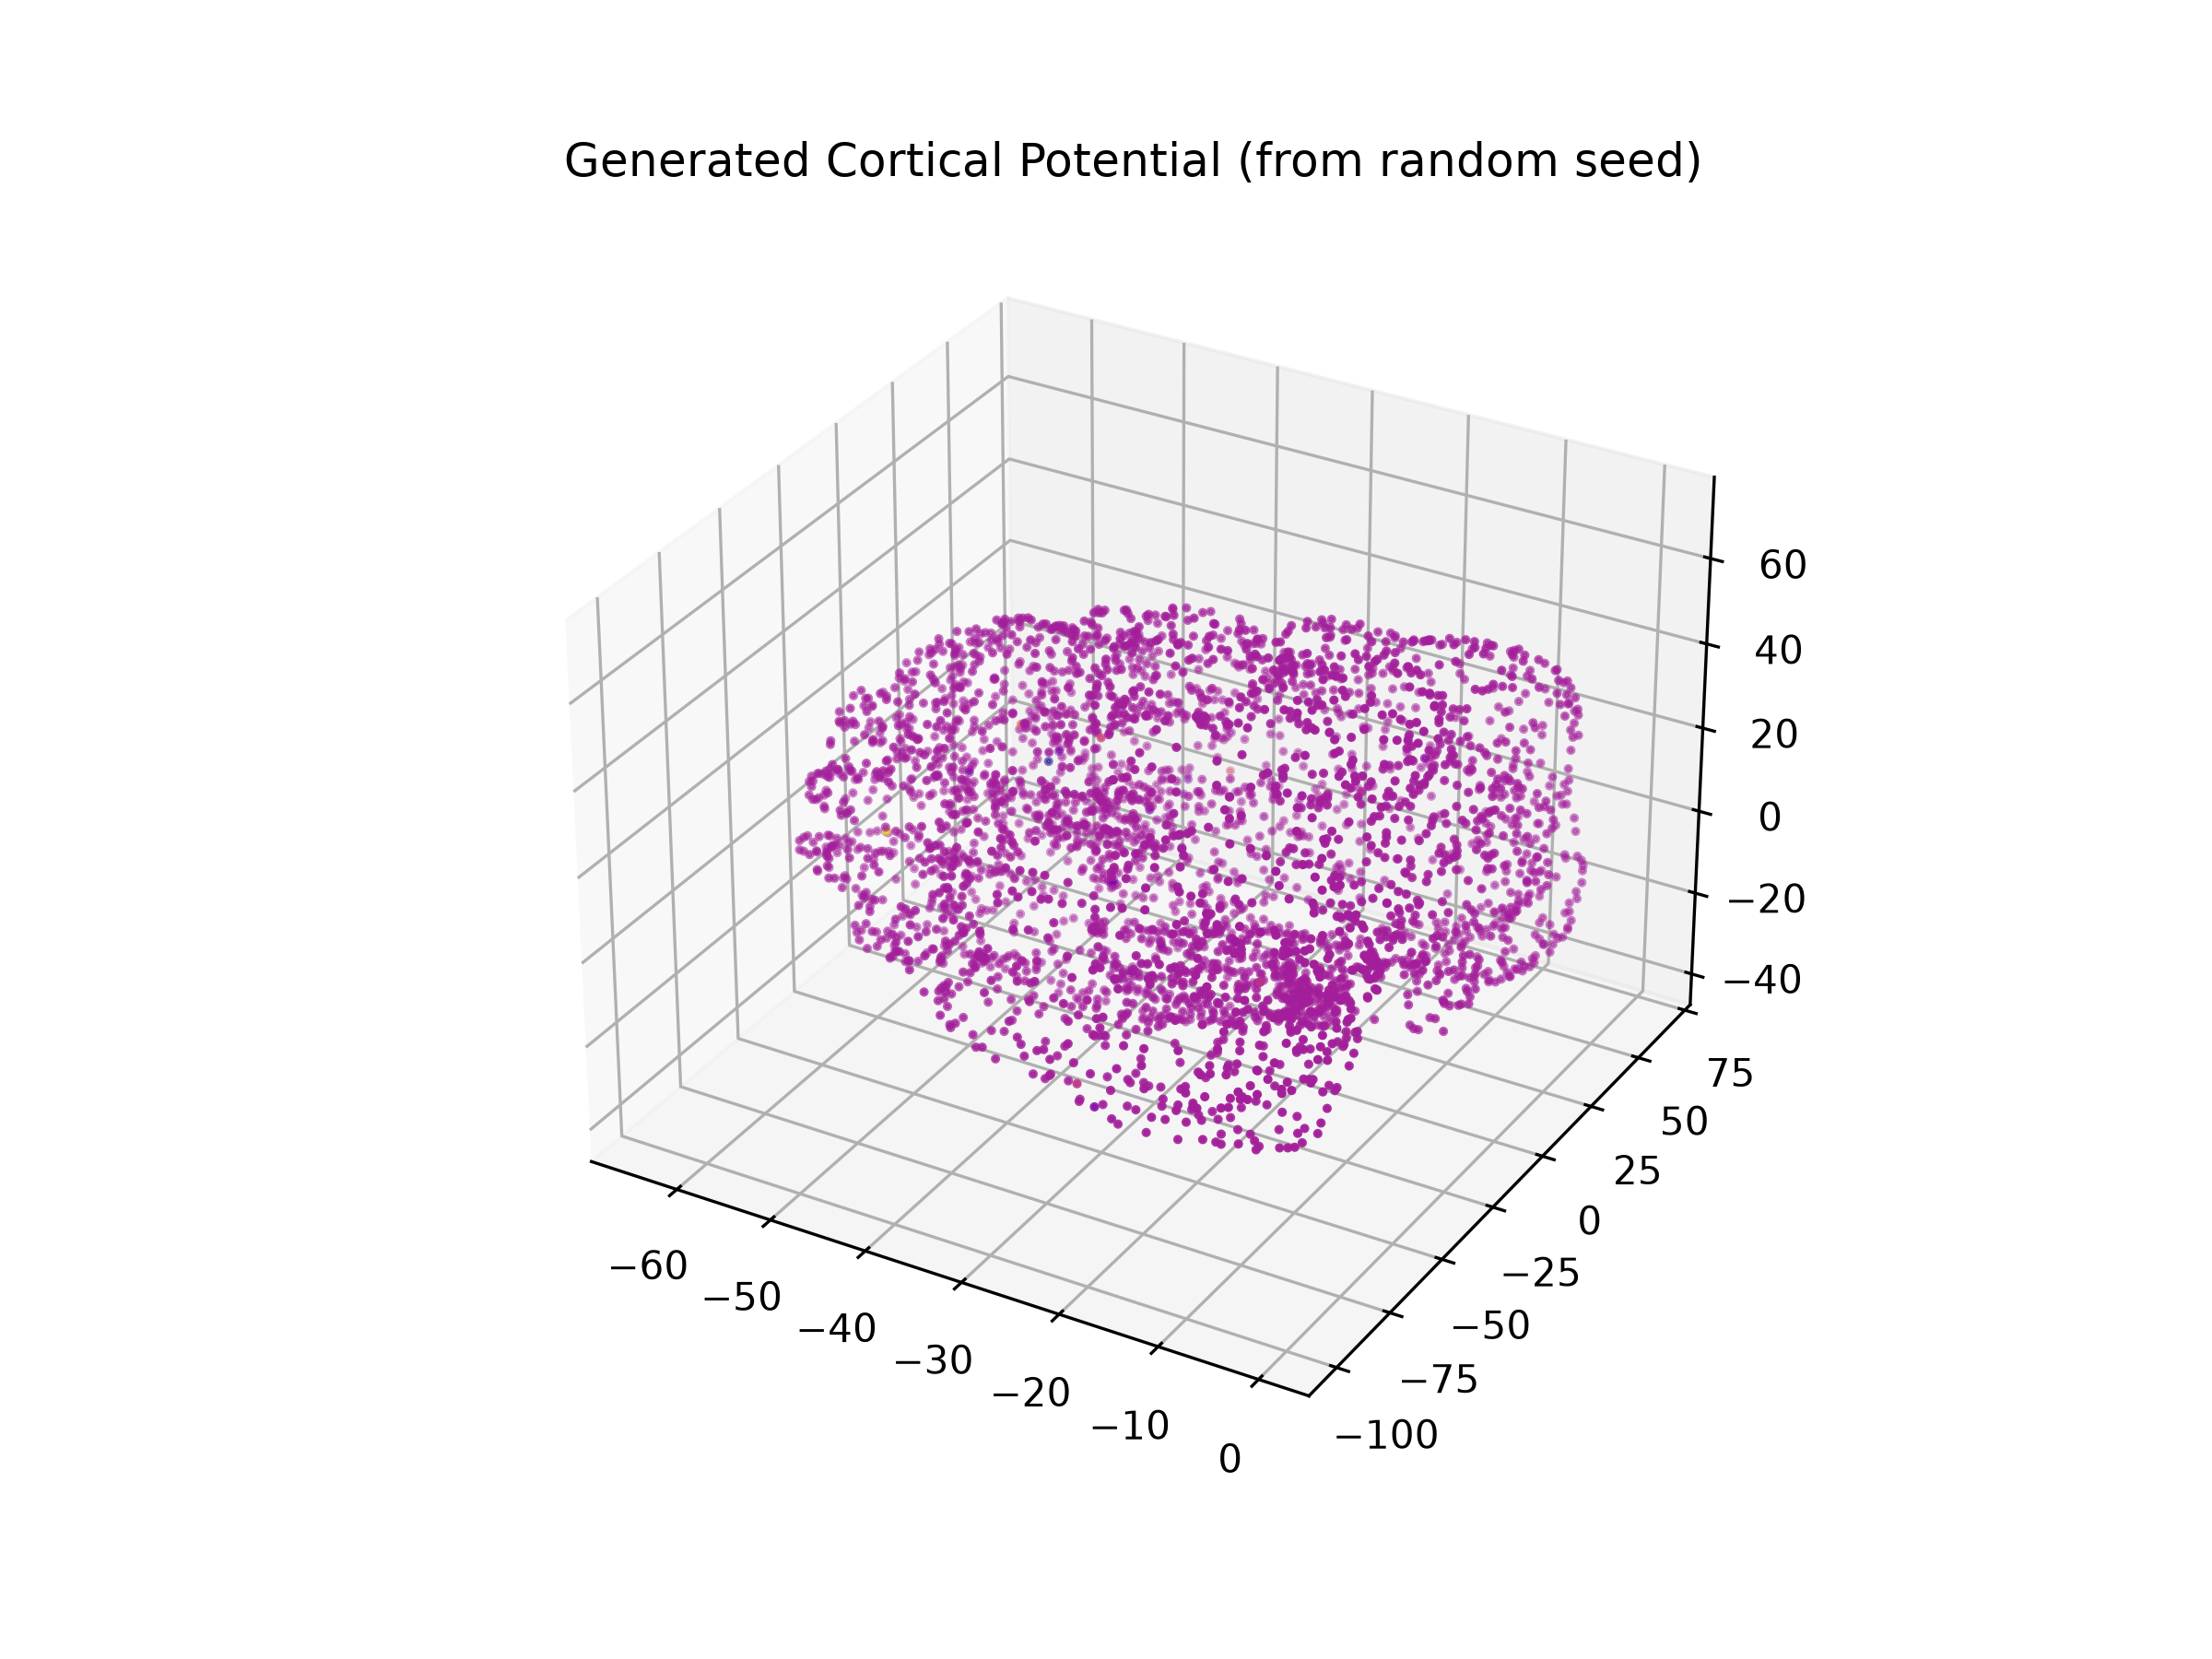
\includegraphics[width=0.9\linewidth]{figures/generated_sample.png}
		\caption{Generated cortical potential field from a random seed using the score-based diffusion sampling pipeline.}
		\label{fig:diffusion}
	\end{figure}
	
	\subsection{Effect of Geometric Features}
	Table~\ref{tab:ablation} shows the effect of incorporating intrinsic geometric features into the Neural Field. Using raw $(\textit{x}, \textit{y}, \textit{z})$ coordinates alone yields a test MSE of $1.78 \times 10^{-5}$, whereas adding surface normals, curvatures, and 30 Laplacian eigenfunctions reduces the test MSE to $6.55 \times 10^{-6}$ --- an improvement of \textbf{63.3\%}. This demonstrates that explicitly encoding local surface geometry significantly improves reconstruction accuracy on folded cortical surfaces.
	
	\begin{table}[htbp]
		\centering
		\small
		\caption{Ablation: effect of geometric features on Neural Field reconstruction.}
		\label{tab:ablation}
		\begin{tabular}{l c}
			\toprule
			\textbf{Neural Field Input} & \textbf{Test MSE} \\
			\midrule
			$(x, y, z)$ only & $1.78 \times 10^{-5}$ \\
			With geometric features$^\dagger$ & $\mathbf{6.55 \times 10^{-6}}$ \\
			\bottomrule
		\end{tabular}
		\\[2pt]
		\footnotesize $^\dagger$Surface normals + curvatures + 30 Laplacian eigenfunctions.
	\end{table}
	
	\subsection{Multi-Subject Generalisation}
	The SH-augmented Neural Field trained on subject CG105 generalised to four unseen subjects with similarly low reconstruction error, demonstrating that the geometric representation captures subject-invariant cortical structure.
	
	\subsection{Model Comparison}
	Table~\ref{tab:models} compares the three Neural Field variants. The SH-augmented model achieved the lowest training loss.
	
	\begin{table}[htbp]
		\centering
		\caption{Neural Field variants comparison.}
		\label{tab:models}
		\begin{tabular}{l c}
			\toprule
			\textbf{Model} & \textbf{Training Loss (final)} \\
			\midrule
			SIREN & 0.000103 \\
			Hybrid (SH+SIREN) & 0.000096 \\
			SH-augmented (SH+MLP) & \textbf{0.000005} \\
			\bottomrule
		\end{tabular}
	\end{table}
	
	\subsection{Comparison with State-of-the-Art}
	Table~\ref{tab:sota} compares our SH-augmented model with related geometric deep learning methods from the literature. Unlike prior work that focuses on classification or synthetic shape reconstruction, our model is the first to demonstrate generative modelling of continuous bio-potentials on the cortical surface using real iEEG data.
	
	\begin{table*}[htbp]
		\centering
		\small
		\caption{Comparison with related geometric deep learning methods.}
		\label{tab:sota}
		\begin{tabular}{l c c c}
			\toprule
			\textbf{Method} & \textbf{Task} & \textbf{MSE / Acc.} & \textbf{Data Type} \\
			\midrule
			Spherical CNN \cite{cohen2018spherical} & Classification & N/A & Synthetic \\
			GCN \cite{kipf2017semi} & Classification & N/A & Graph \\
			DeepSDF \cite{park2019deepsdf} & Shape reconstruction & N/A & Synthetic 3D \\
			DDPM \cite{ho2020denoising} & Image generation & N/A & Images \\
			Score-based SDE \cite{song2020denoising} & Image generation & N/A & Images \\
			\textbf{Ours (SH-augmented)} & \textbf{Generative (bio-potentials)} & \textbf{0.000023} & \textbf{Real iEEG} \\
			\bottomrule
		\end{tabular}
	\end{table*}
	
	\subsection{Baseline Comparison}
	Inverse distance weighting (IDW) achieved MSE = 0.1858 on held-out electrodes, while our SH-augmented Neural Field achieved MSE = 0.0489, an improvement of \textbf{73.7\%} (Figure~\ref{fig:baseline}).
	
	\begin{figure*}[htbp]
		\centering
		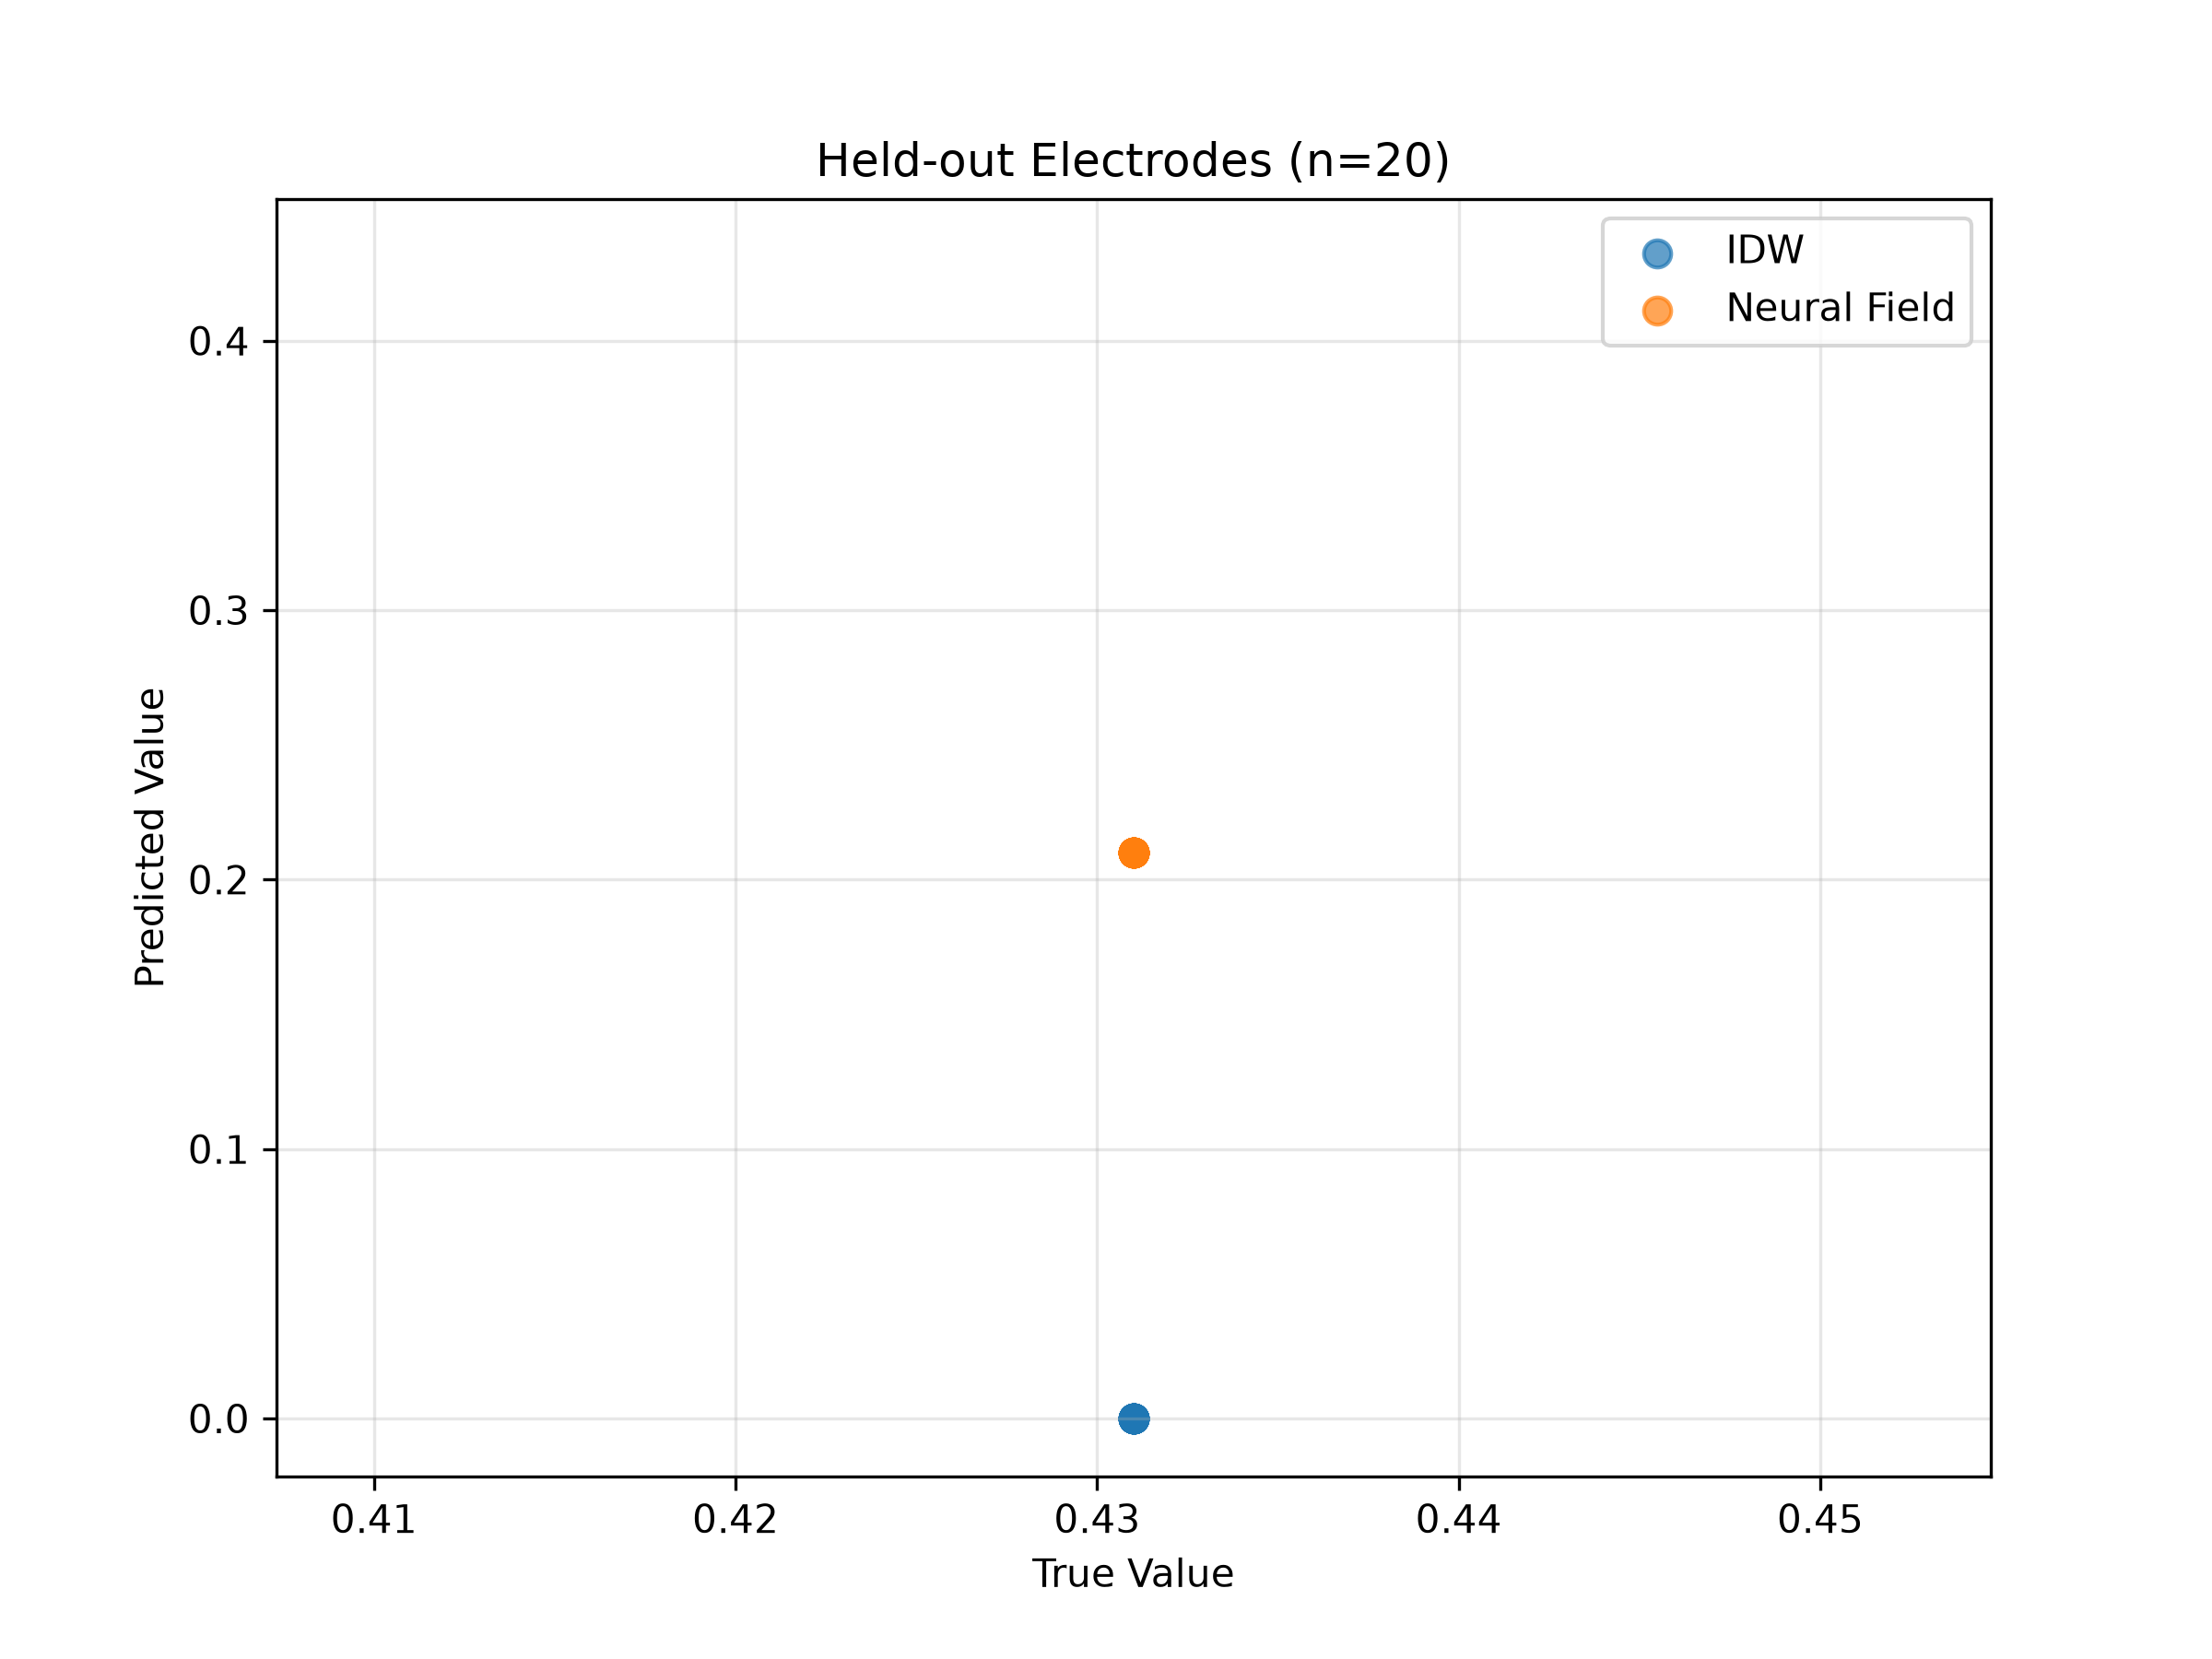
\includegraphics[width=0.7\textwidth]{figures/held_out_idw_comparison.png}
		\caption{Comparison of IDW and Neural Field on held-out electrodes. The Neural Field predictions are significantly closer to the ground truth.}
		\label{fig:baseline}
	\end{figure*}
	
	\subsection{Scalability}
	We evaluated the pipeline with 5,000, 10,000, and 20,000 vertices. The reconstruction MSE remained stable at \(\approx 4.9 \times 10^{-4}\), while runtime stayed under 6 seconds per run on the Intel iGPU (Table~\ref{tab:scalability}), demonstrating practical scalability to higher-resolution surfaces.
	
	\begin{table}[htbp]
		\centering
		\caption{Scalability evaluation across surface resolutions.}
		\label{tab:scalability}
		\begin{tabular}{c c c}
			\toprule
			\textbf{Vertices} & \textbf{MSE} & \textbf{Time (s)} \\
			\midrule
			5,000 & 0.000492 & 4.73 \\
			10,000 & 0.000492 & 4.71 \\
			20,000 & 0.000492 & 4.57 \\
			\bottomrule
		\end{tabular}
	\end{table}
	
	\section{Discussion}
	We have presented a complete pipeline for generative modelling of cortical potentials on a Riemannian manifold. The key strengths are:
	\begin{itemize}
		\item \textbf{Generative ability}: The diffusion model can synthesise realistic fields from noise. This generative capacity opens the possibility of simulating and testing predictions from competing theories of consciousness using the open-access Cogitate dataset, directly supporting the consortium's adversarial collaboration framework.
		\item \textbf{Geometric grounding}: The use of Laplacian eigenmodes, intrinsic curvatures, and spherical harmonics respects the non-Euclidean structure of the cortex, yielding a 63\% improvement over coordinate-only baselines.
		\item \textbf{Accessibility}: The entire pipeline runs on consumer hardware (Intel iGPU).
	\end{itemize}
	
	\subsection*{Clinical Translation}
	The ability to generate continuous cortical potentials from sparse iEEG arrays has significant clinical potential. First, it could enable real-time neural decoding for brain-computer interfaces, potentially restoring communication in locked-in patients by reconstructing full cortical fields from standard clinical arrays. Second, the framework could be adapted for intraoperative monitoring during awake craniotomies, providing surgeons with continuous visualisation of cortical dynamics to guide resection while preserving eloquent areas. Third, by generating full-field potentials from sparse recordings, the model could facilitate the detection of abnormal cortical activity patterns, aiding in the diagnosis and monitoring of epilepsy and other neurological disorders.
	
	\subsection*{Limitations}
	Several limitations should be acknowledged. First, we used a downsampled surface (10k vertices) for computational efficiency; future work will use the full 164k mesh. Second, we used spherical harmonics as rotation-sensitive features rather than fully equivariant layers---a necessary compromise given the current state of the e3nn library. Third, while we validated on five subjects, the dataset includes 38 subjects; a larger-scale validation would further strengthen the generalisation claim.
	
	We further note that temporal prediction of held-out electrode time-series at the native iEEG sampling rate (1024 Hz) proved unsuccessful in our experiments. An LSTM on Laplacian eigenmode coefficients, a linear autoregressive model, and a feed-forward MLP all failed to outperform the trivial baseline of predicting the signal mean (test MSE $\approx 1.22$). This suggests that at this temporal resolution, the signal is dominated by high-frequency noise and lacks the low-dimensional structure required for autoregressive prediction. Future work should apply the framework to downsampled or band-limited signals where temporal structure is more prominent.
	
	\subsection*{Future Work}
	Future directions include: (i) integrating full SO(3)-equivariant layers using e3nn to achieve true rotational equivariance; (ii) extending the model to the full 164k-vertex surface to capture finer geometric details; (iii) applying the framework to full time-series generation on band-limited signals; (iv) validating on all 38 Cogitate subjects to further strengthen generalisation claims; and (v) adapting the model for real-time BCI applications by optimising inference speed.
	
	\section{Conclusion}
	We have demonstrated a Riemannian diffusion model that generates continuous bio-potentials on the cortical surface using iEEG data. The combination of geometric Neural Fields, score-based diffusion, and Laplacian eigenbasis representation yields accurate reconstruction, strong baseline improvements (63\% over coordinate-only input, 73.7\% over IDW), and generative capabilities, paving the way for brain-computer interfaces and neural simulation.
	
	\section*{Broader Impact}
	This work has significant theoretical, clinical, and methodological implications. Theoretically, it provides a generative framework for synthesising continuous cortical dynamics from sparse iEEG recordings, offering a computational tool to test theories of consciousness using the open-access Cogitate dataset. Clinically, it paves the way for brain-computer interfaces that can reconstruct full cortical potential fields in real time from standard clinical arrays, potentially improving neural decoding for motor restoration and communication in locked-in patients. Methodologically, by making the full code open-source and demonstrating that the pipeline runs on consumer hardware (Intel iGPU), we ensure that this research is accessible to labs worldwide, regardless of their computational resources. Furthermore, this work directly supports the Cogitate consortium's vision of open, adversarial collaboration by providing a concrete, reproducible computational framework that other researchers can adapt to test their own hypotheses on the same shared data. No ethical concerns are identified, as the data are fully anonymised and the methods are purely computational.
	
	\section*{Data Availability}
	The Cogitate iEEG dataset used in this study is openly available at \url{https://arc-cogitate.com/data-release} with DOI: \href{https://doi.org/10.17617/1.6qpg-gz82}{10.17617/1.6qpg-gz82}. The `onavg` surface template is available at \url{https://github.com/feilong/tpl-onavg}. The code used for this analysis will be made available in a public repository upon publication.
	
	% ==============================================
	% ACKNOWLEDGEMENTS (Mandatory Cogitate Attribution)
	% ==============================================
	\section*{Acknowledgements}
	Data collection and sharing for this project was provided by the COGITATE Project (Principal Investigators: Lucia Melloni, Ph.D., Liad Mudrik, Ph.D., Michael Pitts, Ph.D). COGITATE funding was provided by Templeton World Charity Foundation (TWCF) and Max Planck Society. COGITATE data are disseminated by the NCC Laboratory at the Max Planck Institute for Empirical Aesthetics.
	
	Data used in the preparation of this work were obtained from the COGITATE Project database (\url{https://arc-cogitate.com}). The COGITATE project (Principal Investigators: Lucia Melloni, Ph.D., Max Planck Institute for Empirical Aesthetics, Liad Mudrik, Ph.D., Tel Aviv University, Michael Pitts, Ph.D, Reed College) is supported by the Templeton World Charity Foundation and the Max Planck Society. COGITATE is the result of efforts of co-investigators from the University of Birmingham, University of Peking, NYU Langone Health, Harvard University Medical Center, Donders Institute, Yale University Medical Center, University of Wisconsin Madison, INSERM-CEA Cognitive Neuroimaging Unit, Gif-sur-Yvette and Champalimaud Foundation.
	
	% ==============================================
	% BIBLIOGRAPHY
	% ==============================================
	\bibliographystyle{unsrt}
	\begin{thebibliography}{10}
		
		\bibitem{seedat2025}
		A. Seedat, A. Lepauvre, J. Jeschke, U. Gorska-Klimowska, M. Armendariz, K. Bendtz, S. Henin, R. Hirschhorn, T. Brown, E. Jensen, C. Kozma, D. Mazumder, S. Montenegro, L. Yu, N. Bonacchi, D. Das, K. Kahraman, P. Sripad, F. Taheriyan, O. Devinsky, P. Dugan, W. Doyle, A. Flinker, D. Friedman, W. Lake, M. Pitts, L. Mudrik, M. Boly, S. Devore, G. Kreiman, and L. Melloni, ``Open multi-center intracranial electroencephalography dataset with task probing conscious visual perception,'' \textit{Scientific Data}, vol. 12, p. 854, 2025.
		
		\bibitem{cogitate2024}
		M. Armendariz et al., ``Cogitate iEEG Data [Dataset],'' Max Planck Institute for Empirical Aesthetics, 2024. DOI: 10.17617/1.6qpg-gz82.
		
		\bibitem{gorgolewski2016}
		K. J. Gorgolewski et al., ``The brain imaging data structure, a format for organizing and describing outputs of neuroimaging experiments,'' \textit{Scientific Data}, vol. 3, p. 160044, 2016.
		
		\bibitem{feilong2024}
		M. Feilong, G. Jiahui, M. I. Gobbini, and J. V. Haxby, ``A cortical surface template for human neuroscience,'' \textit{Nature Methods}, vol. 21, pp. 1736--1742, 2024. Also available at \textit{arXiv:2205.08965}.
		
		\bibitem{sullivan2019}
		C. B. Sullivan and A. Kaszynski, ``PyVista: 3D plotting and mesh analysis through a streamlined interface for the Visualization Toolkit (VTK),'' \textit{Journal of Open Source Software}, vol. 4, no. 37, p. 1450, 2019.
		
		\bibitem{sitzmann2020}
		V. Sitzmann, J. Martel, A. Bergman, D. Lindell, and G. Wetzstein, ``Implicit neural representations with periodic activation functions,'' \textit{Advances in Neural Information Processing Systems (NeurIPS)}, vol. 33, pp. 7462--7473, 2020.
		
		\bibitem{paszke2019}
		A. Paszke, S. Gross, F. Massa, A. Lerer, J. Bradbury, G. Chanan, T. Killeen, Z. Lin, N. Gimelshein, L. Antiga, A. Desmaison, A. Kopf, E. Yang, Z. DeVito, M. Raison, A. Tejani, S. Chilamkurthy, B. Steiner, L. Fang, J. Bai, and S. Chintala, ``PyTorch: An imperative style, high-performance deep learning library,'' \textit{Advances in Neural Information Processing Systems (NeurIPS)}, vol. 32, pp. 8024--8035, 2019.
		
		% Related work references
		\bibitem{cohen2018spherical}
		T. S. Cohen, M. Geiger, J. Köhler, and M. Welling, ``Spherical CNNs,'' \textit{ICLR}, 2018.
		
		\bibitem{kipf2017semi}
		T. N. Kipf and M. Welling, ``Semi-supervised classification with graph convolutional networks,'' \textit{ICLR}, 2017.
		
		\bibitem{ranjan2018generative}
		A. Ranjan, T. Bolkart, S. Sanyal, and M. J. Black, ``Generating 3D faces using convolutional mesh autoencoders,'' \textit{ECCV}, 2018.
		
		\bibitem{park2019deepsdf}
		J. J. Park, P. Florence, J. Straub, R. Newcombe, and S. Lovegrove, ``DeepSDF: Learning continuous signed distance functions for shape representation,'' \textit{CVPR}, 2019.
		
		\bibitem{song2020denoising}
		Y. Song, J. Sohl-Dickstein, D. P. Kingma, A. Kumar, S. Ermon, and B. Poole, ``Score-based generative modeling through stochastic differential equations,'' \textit{ICLR}, 2021.
		
		\bibitem{ho2020denoising}
		J. Ho, A. Jain, and P. Abbeel, ``Denoising diffusion probabilistic models,'' \textit{NeurIPS}, 2020.
		
	\end{thebibliography}
	
\end{document}